\documentclass[10pt,hyperref={colorlinks,citecolor=blue,urlcolor=peking_blue,linkcolor=}]{beamer}
\usepackage{PekingU}
\usefonttheme{serif}
\usepackage{lipsum}
\usepackage{hyperref}
\usepackage{charter} % Nicer fonts
\usepackage{latexsym,amsmath,xcolor,multicol,booktabs,calligra}
\usepackage{amssymb}
\usepackage{graphicx}
\usepackage{bm}
\usepackage{natbib}
\usepackage{wrapfig}
\usepackage{amsfonts} 
\usepackage{ragged2e}
\usepackage{parskip}
\apptocmd{\frame}{}{\justifying}{} % Allow optional arguments after frame.
\newcommand{\theHalgorithm}{\arabic{algorithm}}
\theoremstyle{plain}
\newtheorem{axiom}{Axiom}
\newtheorem{claim}[axiom]{Claim}
\newtheorem{assumption}{Assumption}
\newtheorem{remark}{Remark}
\newtheorem{proposition}{Proposition}
\setbeamertemplate{theorems}[numbered]


\author[Pei Feng Tong]{Pei Feng Tong}
\title{Peking University Beamer Template}
\subtitle{lightweight designed}
\institute{Guanghua School of Management, Peking University}
\date{
2024/01/15}

\newif\ifplacelogo % create a new conditional
\placelogotrue % set it to true
\logo{
\ifplacelogo
\includegraphics[width=2cm]{../Figures/PKU-China-logo.png}
\fi
}
% official colors match with the PKU red
\def\cmd#1{\texttt{\color{red}\footnotesize $\backslash$#1}}
\def\env#1{\texttt{\color{blue}\footnotesize #1}}
\definecolor{deepblue}{rgb}{0,0,0.5}
\definecolor{deepred}{rgb}{0.6,0,0}
\definecolor{deepgreen}{rgb}{0,0.5,0}
\definecolor{halfgray}{gray}{0.55}

\begin{document}
{
\setbeamertemplate{logo}{}
\begin{frame}
    \titlepage
    \begin{figure}[htpb]
        \begin{center}
            \includegraphics[width=0.2\linewidth]{Figures/PKUlogo.png}
        \end{center}
    \end{figure}
\end{frame}
}

\placelogofalse

\section{Introduction}
\begin{frame}{Background}
\begin{figure}[Visit to Auburn Lab in Alabama]
\begin{center}
\includegraphics[width=1\linewidth]{../Figures/Misc/infrontofthemachine.png}
\end{center}
\end{figure}
\begin{enumerate}
\item Collaborating with USDA Agriculture Research Service
\item Developing an in situ spectroscopy device for soil analysis
\end{enumerate}
\end{frame}
\begin{frame}{Core Harvesting}
\begin{figure}[Core Harvest]
\begin{center}
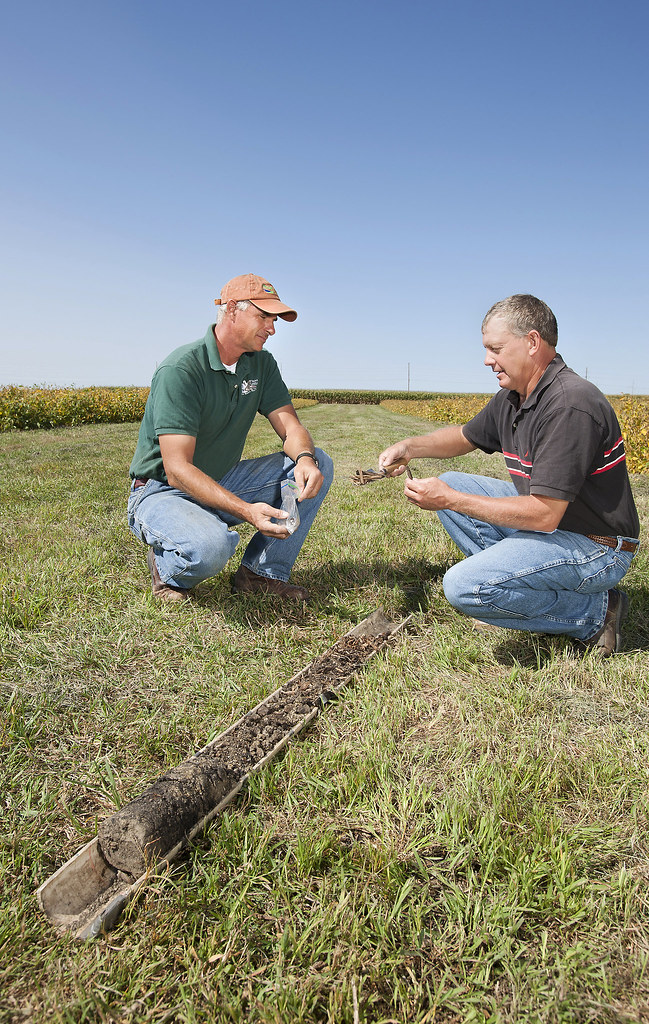
\includegraphics[width=1\linewidth]{../Figures/Misc/SoilCore.jpg}
\end{center}
\end{figure}
\begin{enumerate}
\item Traditional method: “Core Harvesting”
\item Large soil cores extracted and analyzed in lab
\item Time-consuming, labor-intensive
\end{enumerate}
\end{frame}
\begin{frame}{In Situ Spectroscopy Device}
\begin{figure}[MINS on Field]
\begin{center}
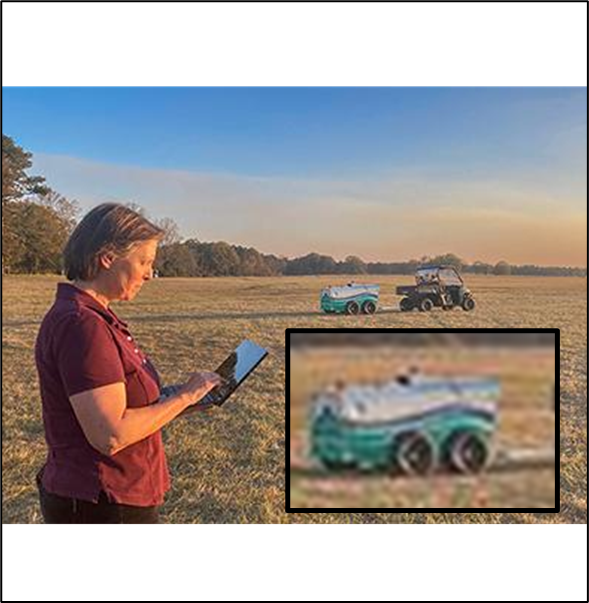
\includegraphics[width=1\linewidth]{../Figures/Misc/MINSInField.png}
\end{center}
\end{figure}
\begin{enumerate}
\item Fast, nondestructive, cost-effective alternative
\item “Mobile Inelastic Neutron Scattering System”
\item Uses gamma ray spectroscopy to measure soil composition directly
\end{enumerate}
\end{frame}
\begin{frame}{Simulation is done in MCNP}
\begin{enumerate}
\item My role: Mathematical support and simulation
\item Analyze and generate spectroscopy results
Simulations performed in MCNP6.2
\item Presenting challenges addressed with MCNP
\end{enumerate}
\end{frame}
\section{Soil in MCNP}
\begin{frame}{Soil is a Nonhomogenous Material}
\begin{figure}[Carbon case study over a field]
\begin{center}
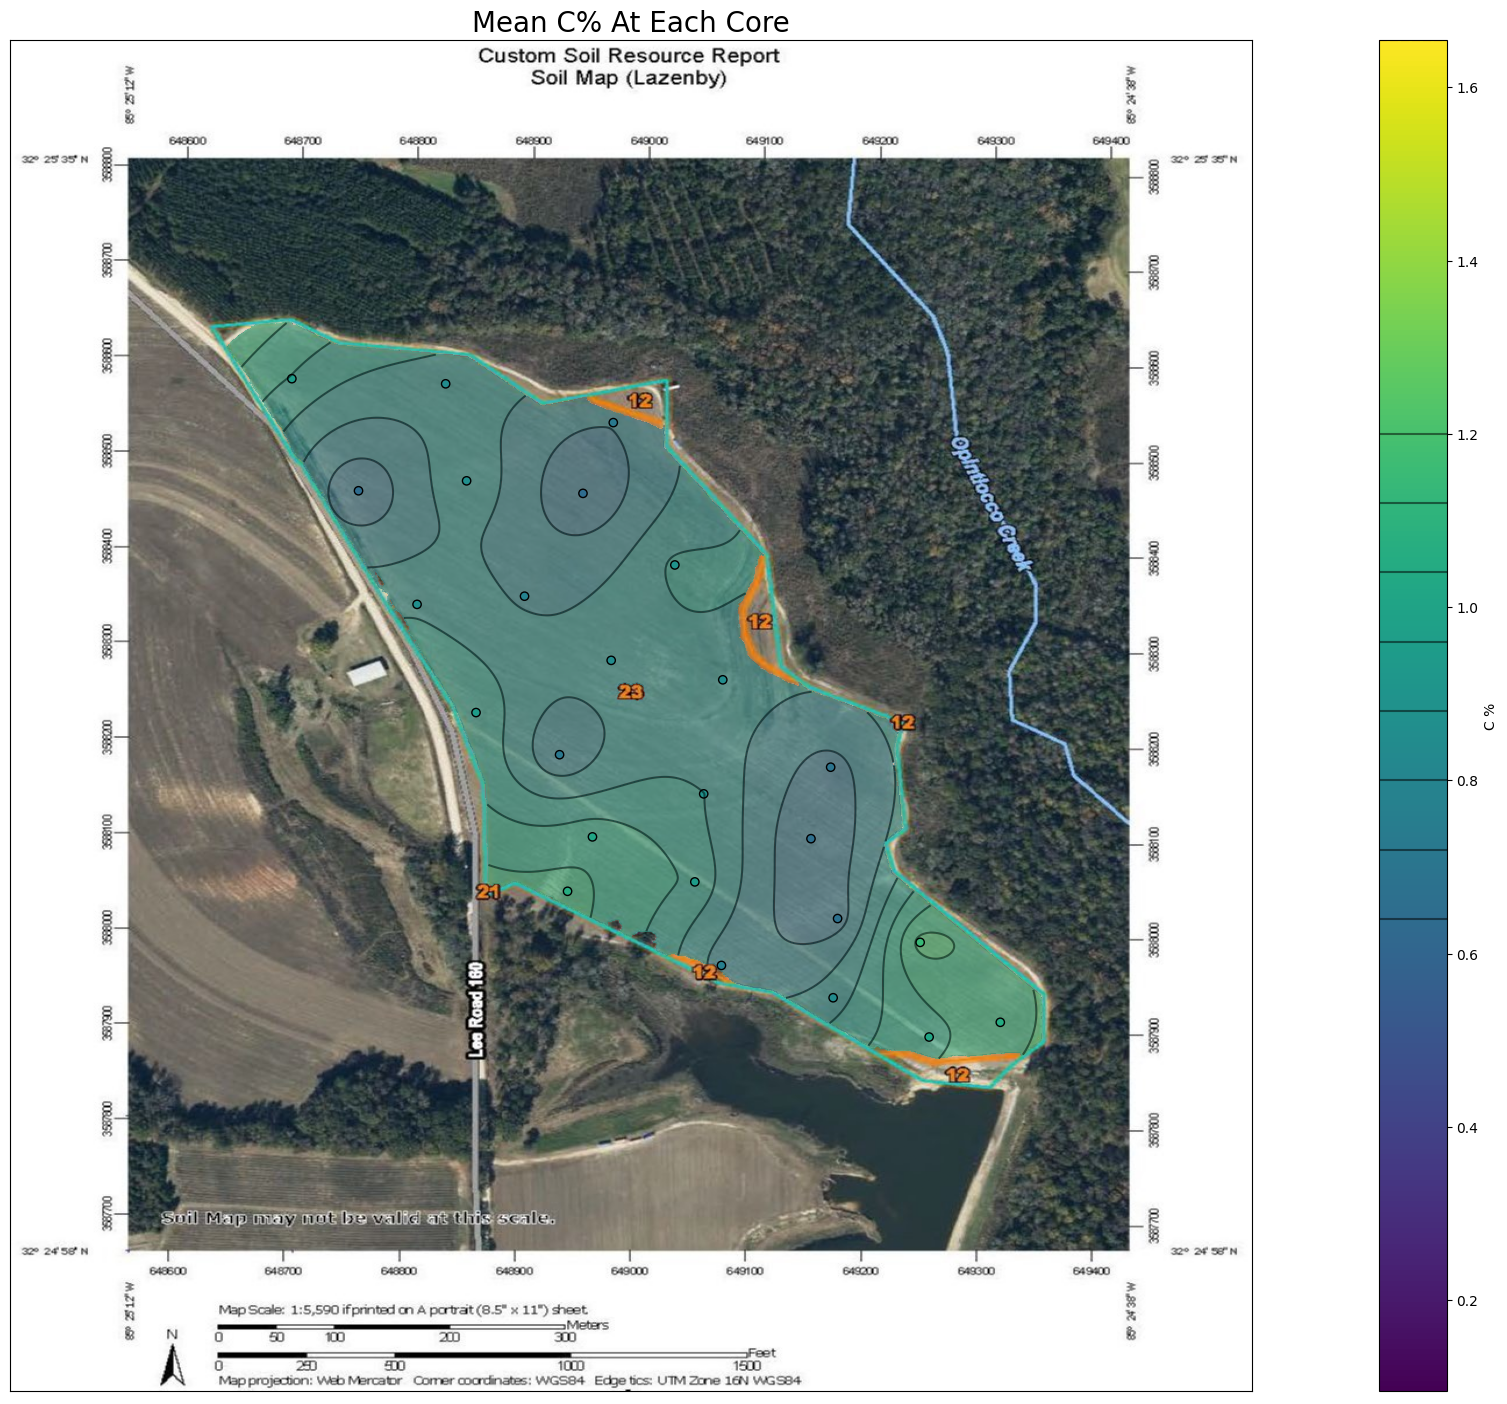
\includegraphics[width=1\linewidth]{../Figures/CaseStudy/fieldstudy.png}
\end{center}
\end{figure}
\begin{figure}[Carbon case study over depth]
\begin{center}
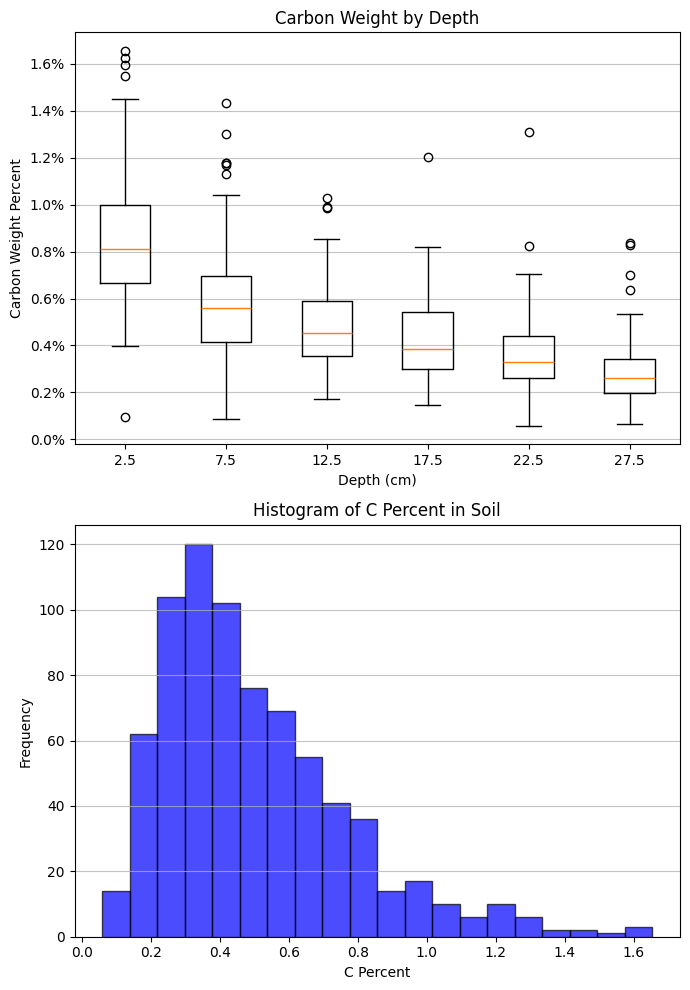
\includegraphics[width=1\linewidth]{../Figures/CaseStudy/depthstudy.png}
\end{center}
\end{figure}
\begin{enumerate}
\item MCNP cells assume homogeneous material
Real soil: heterogeneous at many scales
\item Carbon often decreases exponentially with depth
\end{enumerate}
\end{frame}
\begin{frame}{Functionally Defined Soil}
\begin{figure}[Carbon as a function in the soil]
\begin{center}
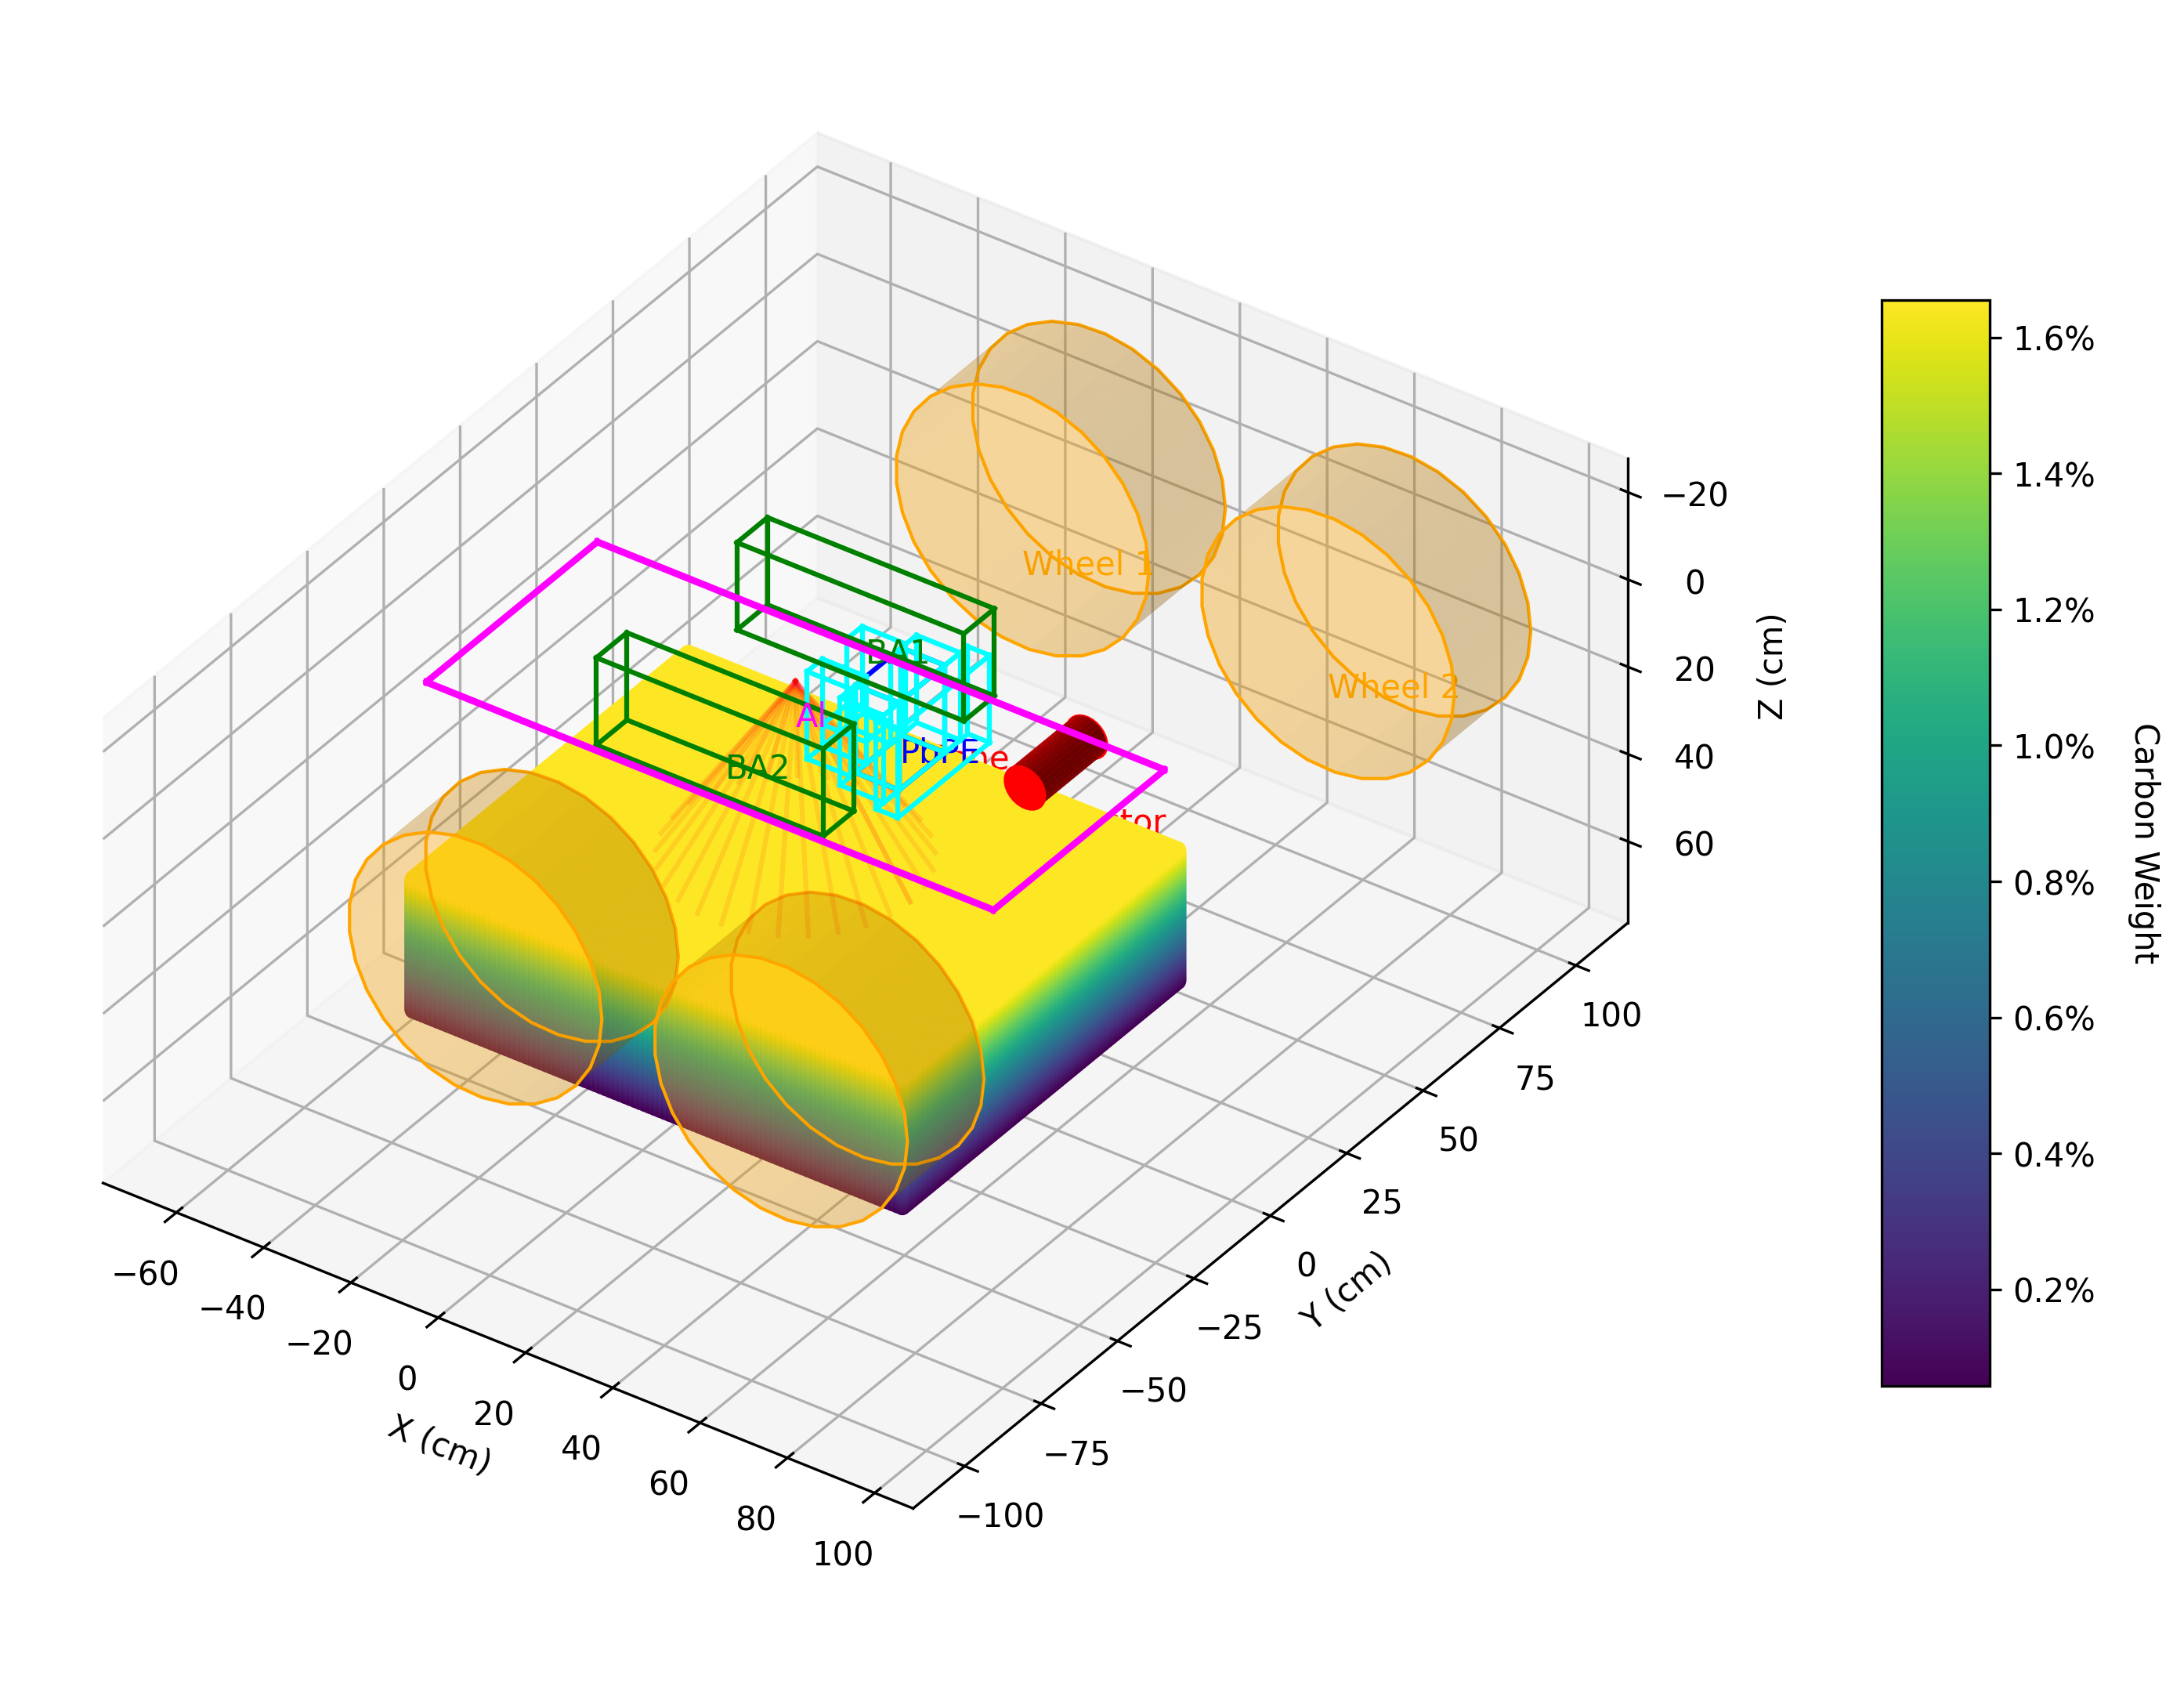
\includegraphics[width=1\linewidth]{../Figures/FunctionallyDefinedSoil/Carbonasafunctioninthesoil.png}
\end{center}
\end{figure}
\begin{enumerate}
\item Soil characteristics can be described as functions of 3D space
\item Needed a way to translate this into MCNP input
\end{enumerate}
\end{frame}
\begin{frame}{Mesh Cells}
\begin{figure}[Single to many cells]
\begin{center}
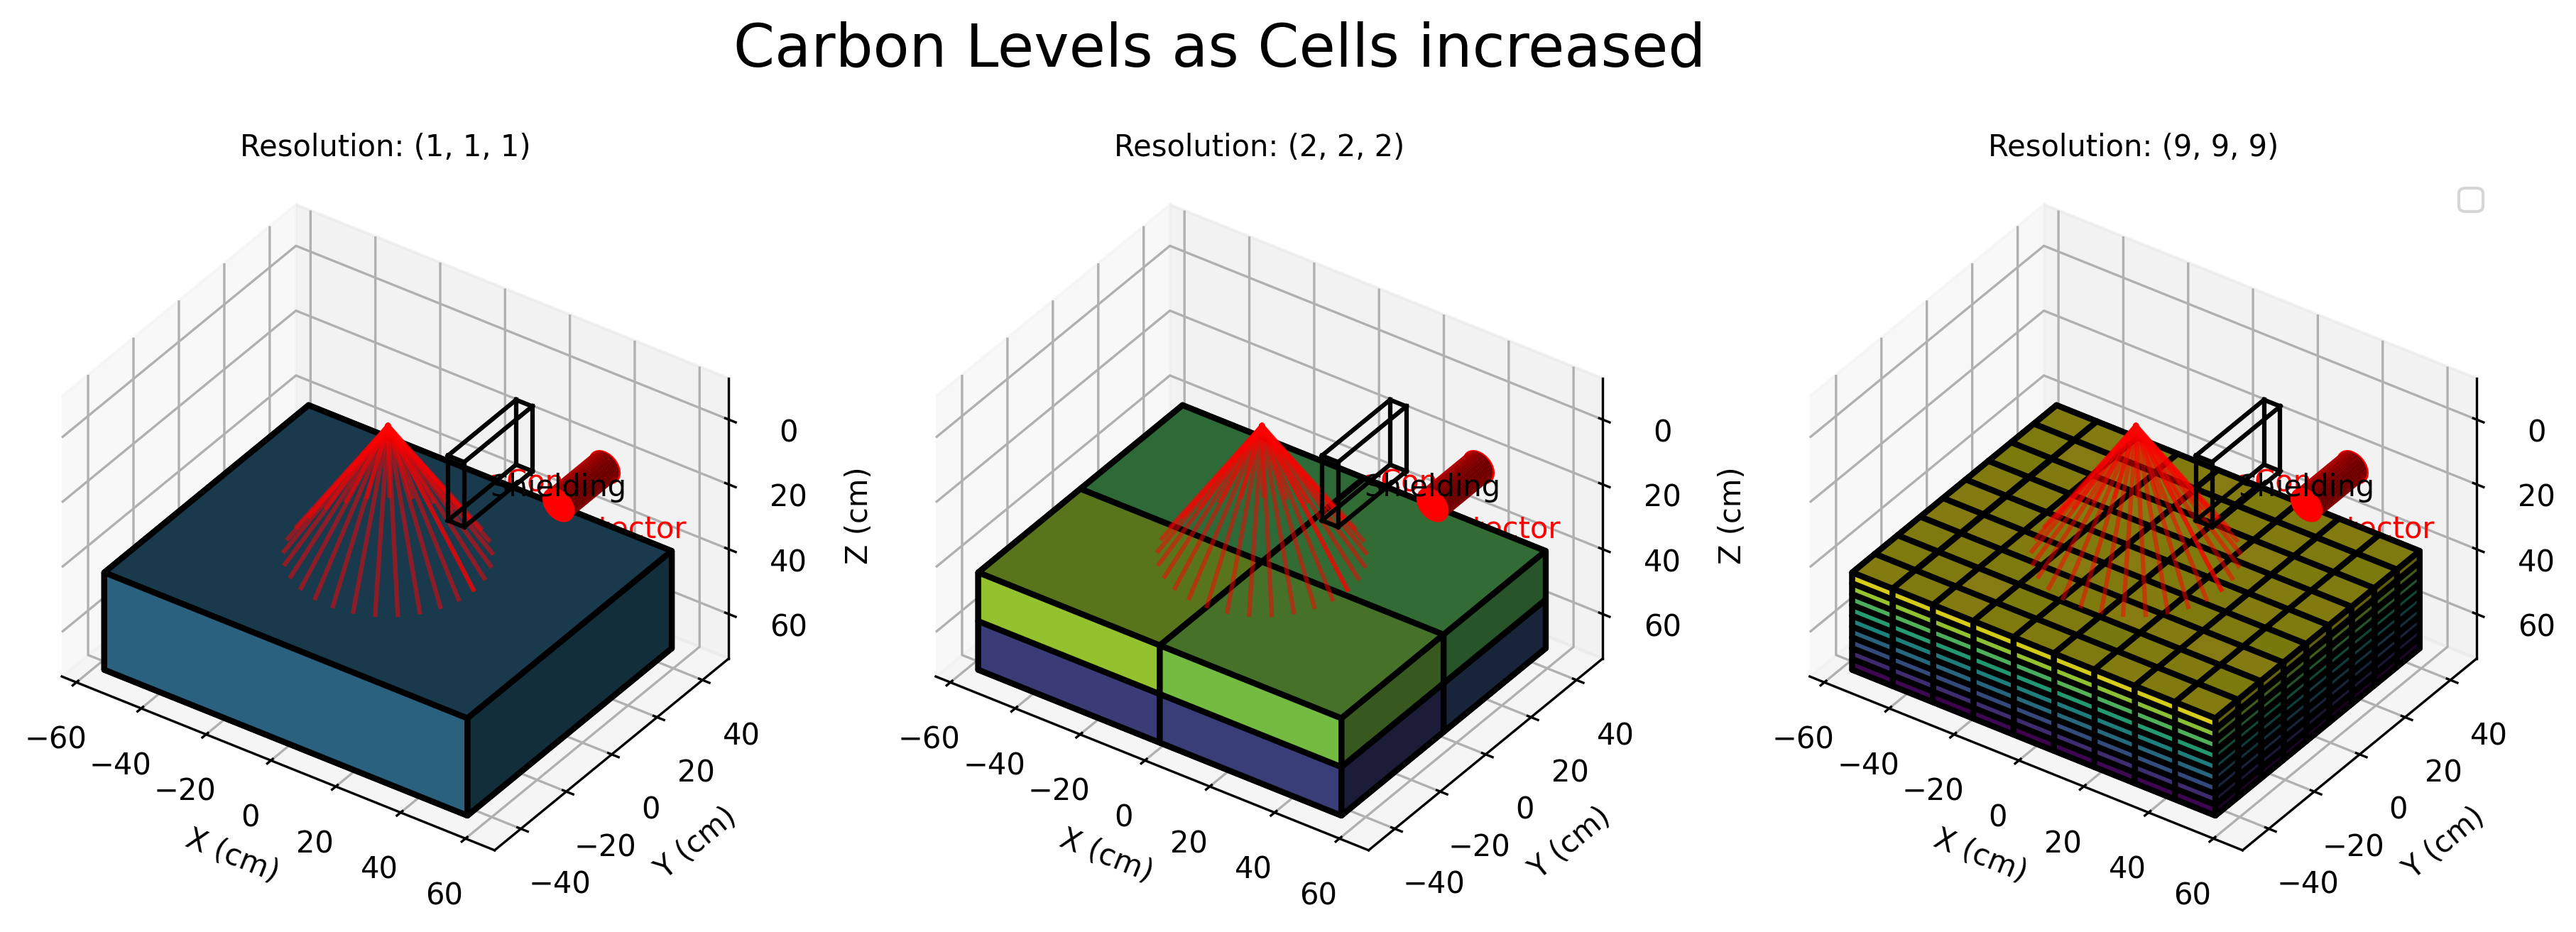
\includegraphics[width=1\linewidth]{../Figures/MCNP/SingleToManyCells.png}
\end{center}
\end{figure}
\begin{enumerate}
\item Divide soil into a mesh of smaller cells
Approximate functional characteristics in discrete space
\item Higher mesh resolution = more accurate representation
\end{enumerate}
\end{frame}
\begin{frame}{Defining cell characteristics}
\begin{figure}[Individual Cell Sampling]
\begin{center}
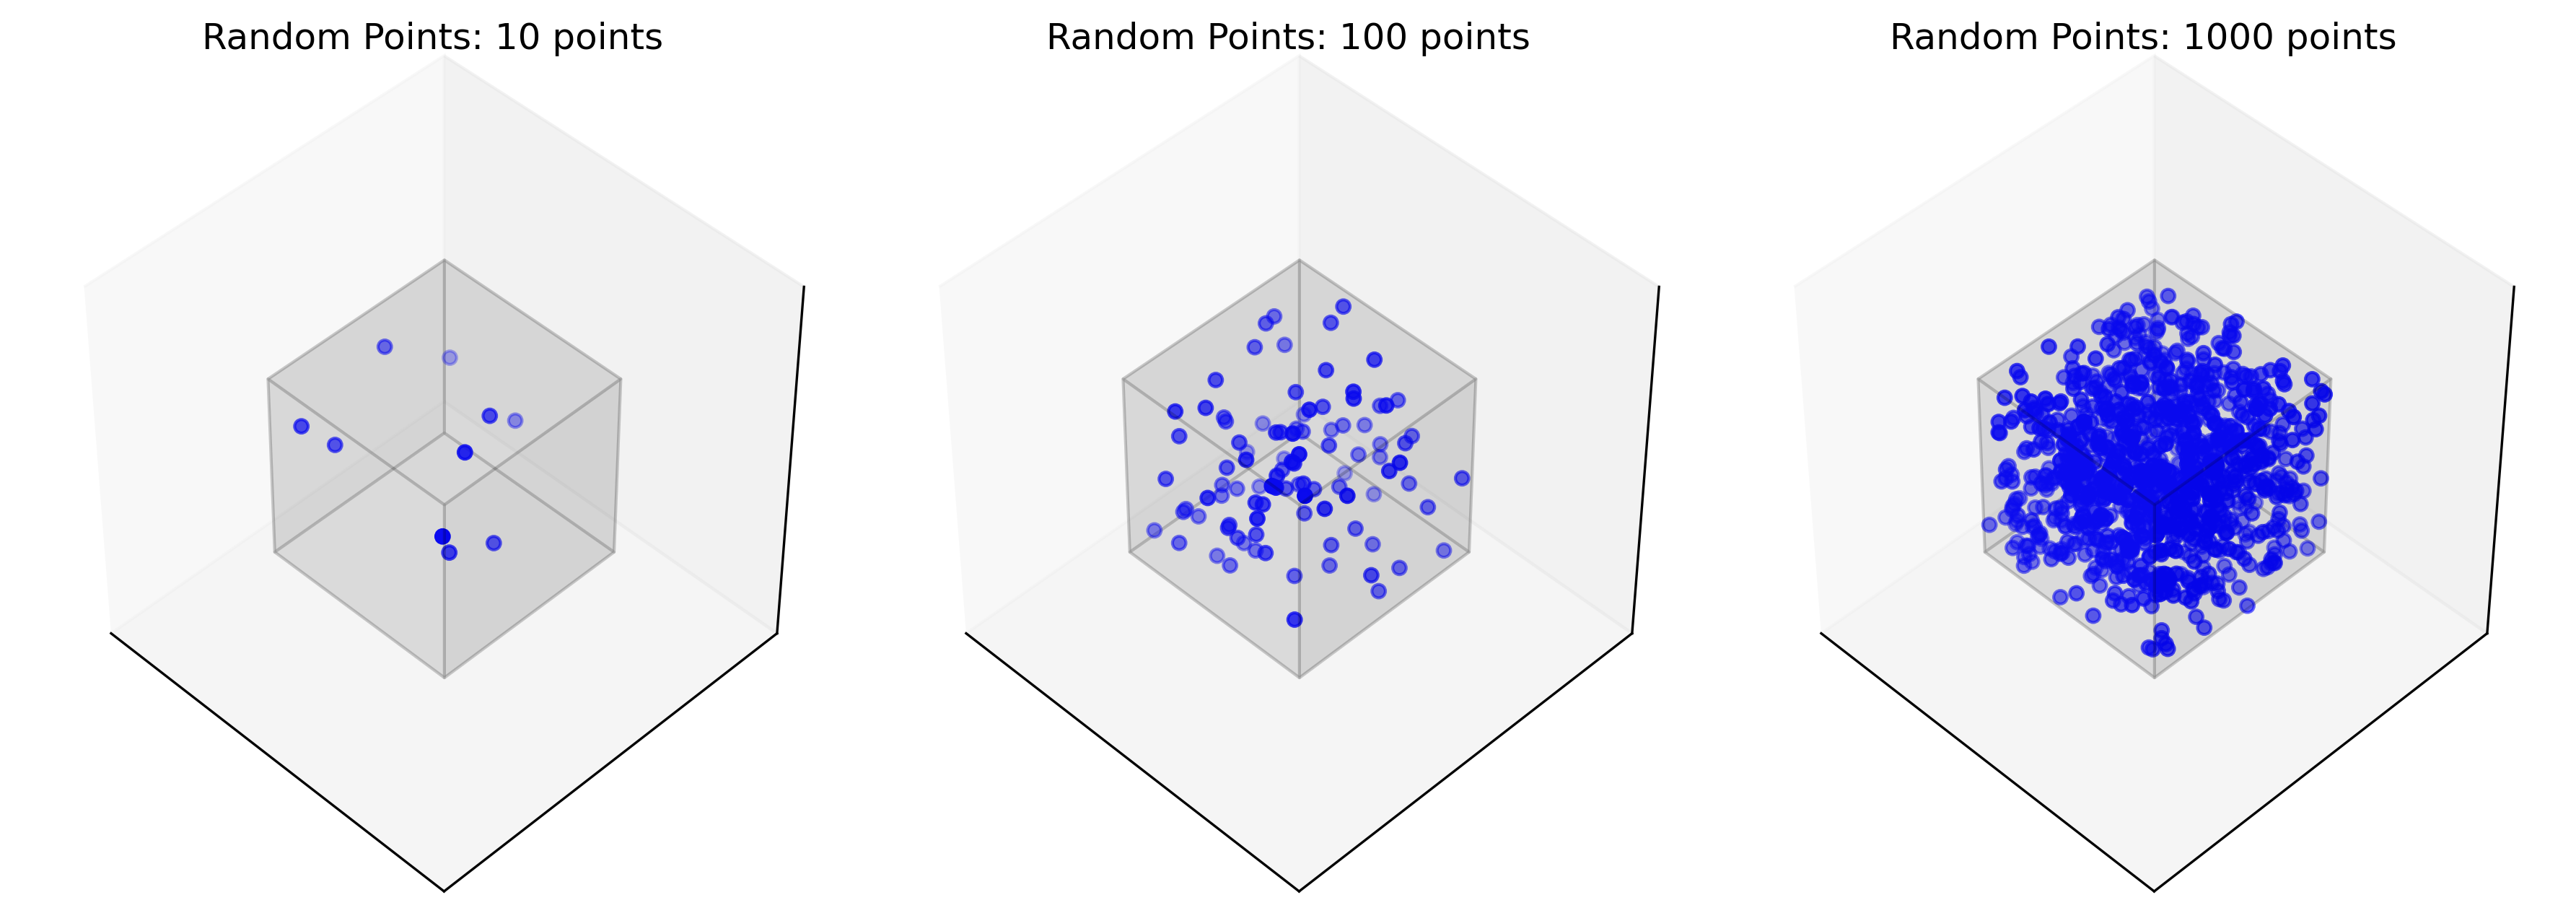
\includegraphics[width=1\linewidth]{../Figures/FunctionallyDefinedSoil/IndividualCellSampling.png}
\end{center}
\end{figure}
\begin{enumerate}
\item Use Monte Carlo sampling to average properties in each mesh cell
\item Assign average values to each cell
Results in a more detailed, accurate soil mode
\end{enumerate}
\end{frame}
\section{Results}
\begin{frame}{effects on detection}
\begin{figure}[Effects of resolution on detection]
\begin{center}
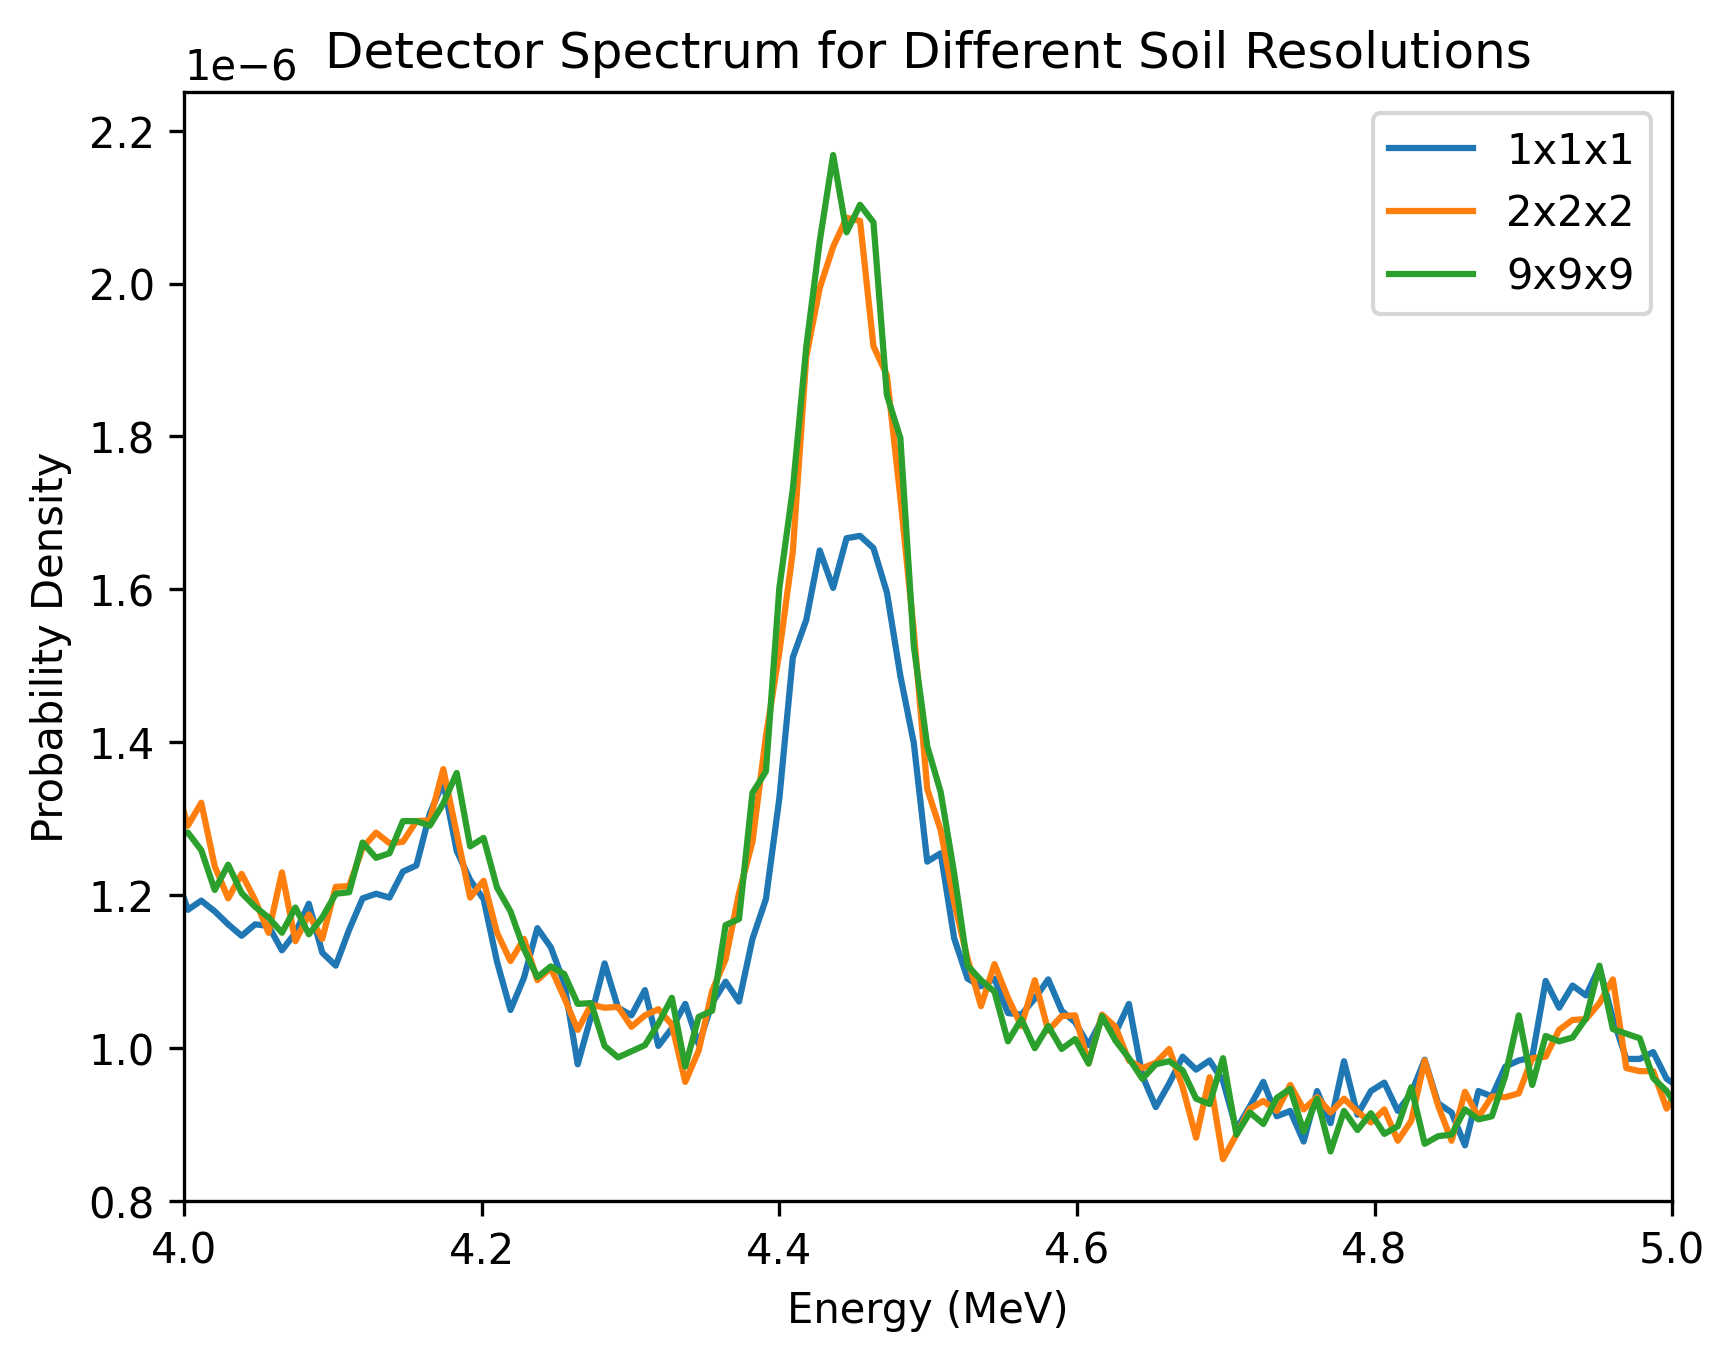
\includegraphics[width=1\linewidth]{../Figures/MCNP/Effectsofresolutionondetection.png}
\end{center}
\end{figure}
\begin{enumerate}
\item Start with a homogeneous cell, then subdivide
\item As mesh resolution increases, carbon density approaches true function
\item Spectral readings become more accurate
\item Readings are sensitive to local variations
\end{enumerate}
\end{frame}
\begin{frame}{Soil is a Semi-Infinite Sample}
\begin{figure}[Lab Spectroscopy]
\begin{center}
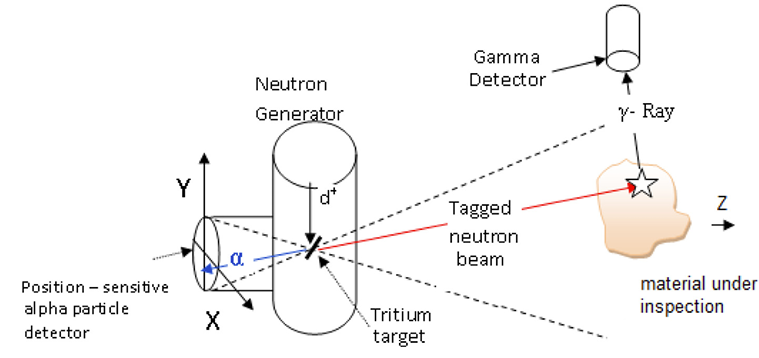
\includegraphics[width=1\linewidth]{../Figures/Misc/LabSpectros.png}
\end{center}
\end{figure}
\begin{figure}[Field Spectroscopy]
\begin{center}
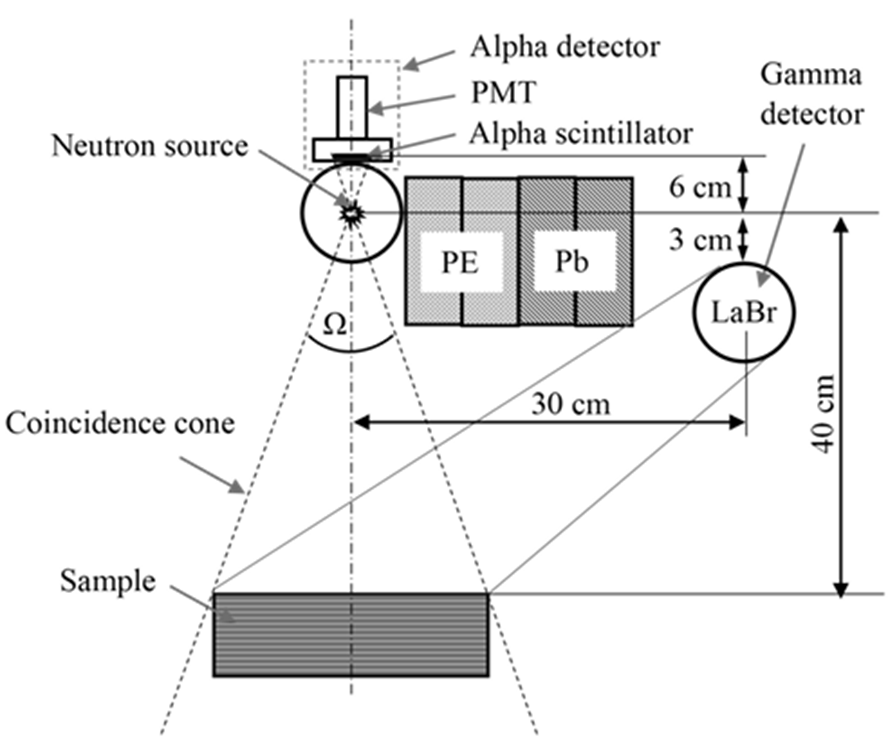
\includegraphics[width=1\linewidth]{../Figures/Misc/FieldSpectros.png}
\end{center}
\end{figure}
\begin{enumerate}
\item Investigate detection range of the device
\item Lab: detector covers entire sample
\item Field: soil is semi-infinite, detection range is finite
\end{enumerate}
\end{frame}
\begin{frame}{Cell Mesh vs FMESH}
\begin{figure}[Cell Mesh vs FMESH code]
\begin{center}
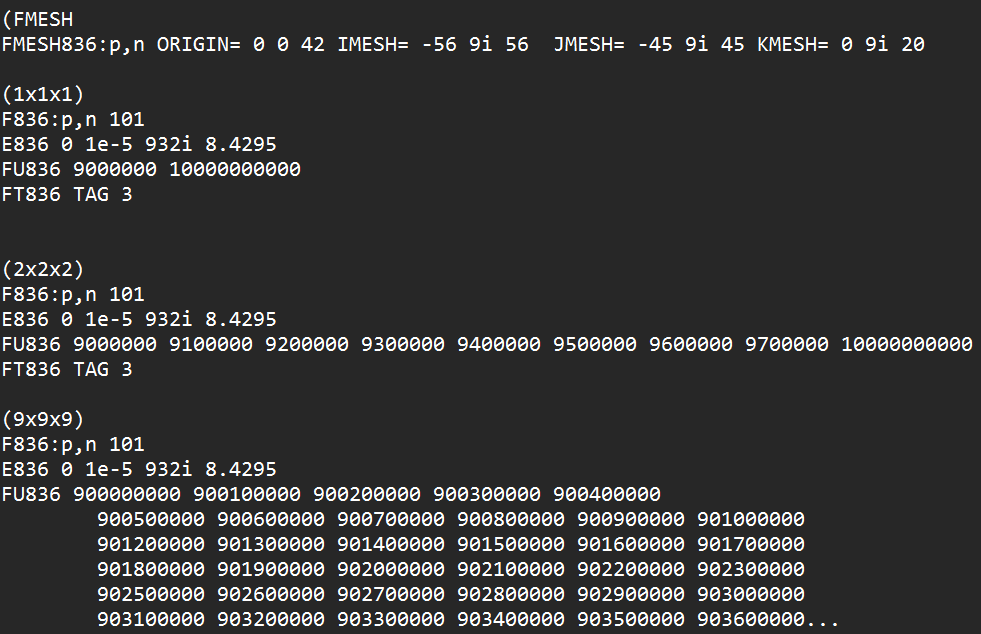
\includegraphics[width=1\linewidth]{../Figures/MCNP/maxfmesh.png}
\end{center}
\end{figure}
\begin{enumerate}
\item MCNP FMESH: tally results in mesh bins (for imaging, range studies)
\item Cell meshes: can also tally per cell
\item Both methods help analyze detection range
\end{enumerate}
\end{frame}
\begin{frame}{Independent Cell Functionality}
\begin{figure}[Cell Ratio Mesh Detection]
\begin{center}
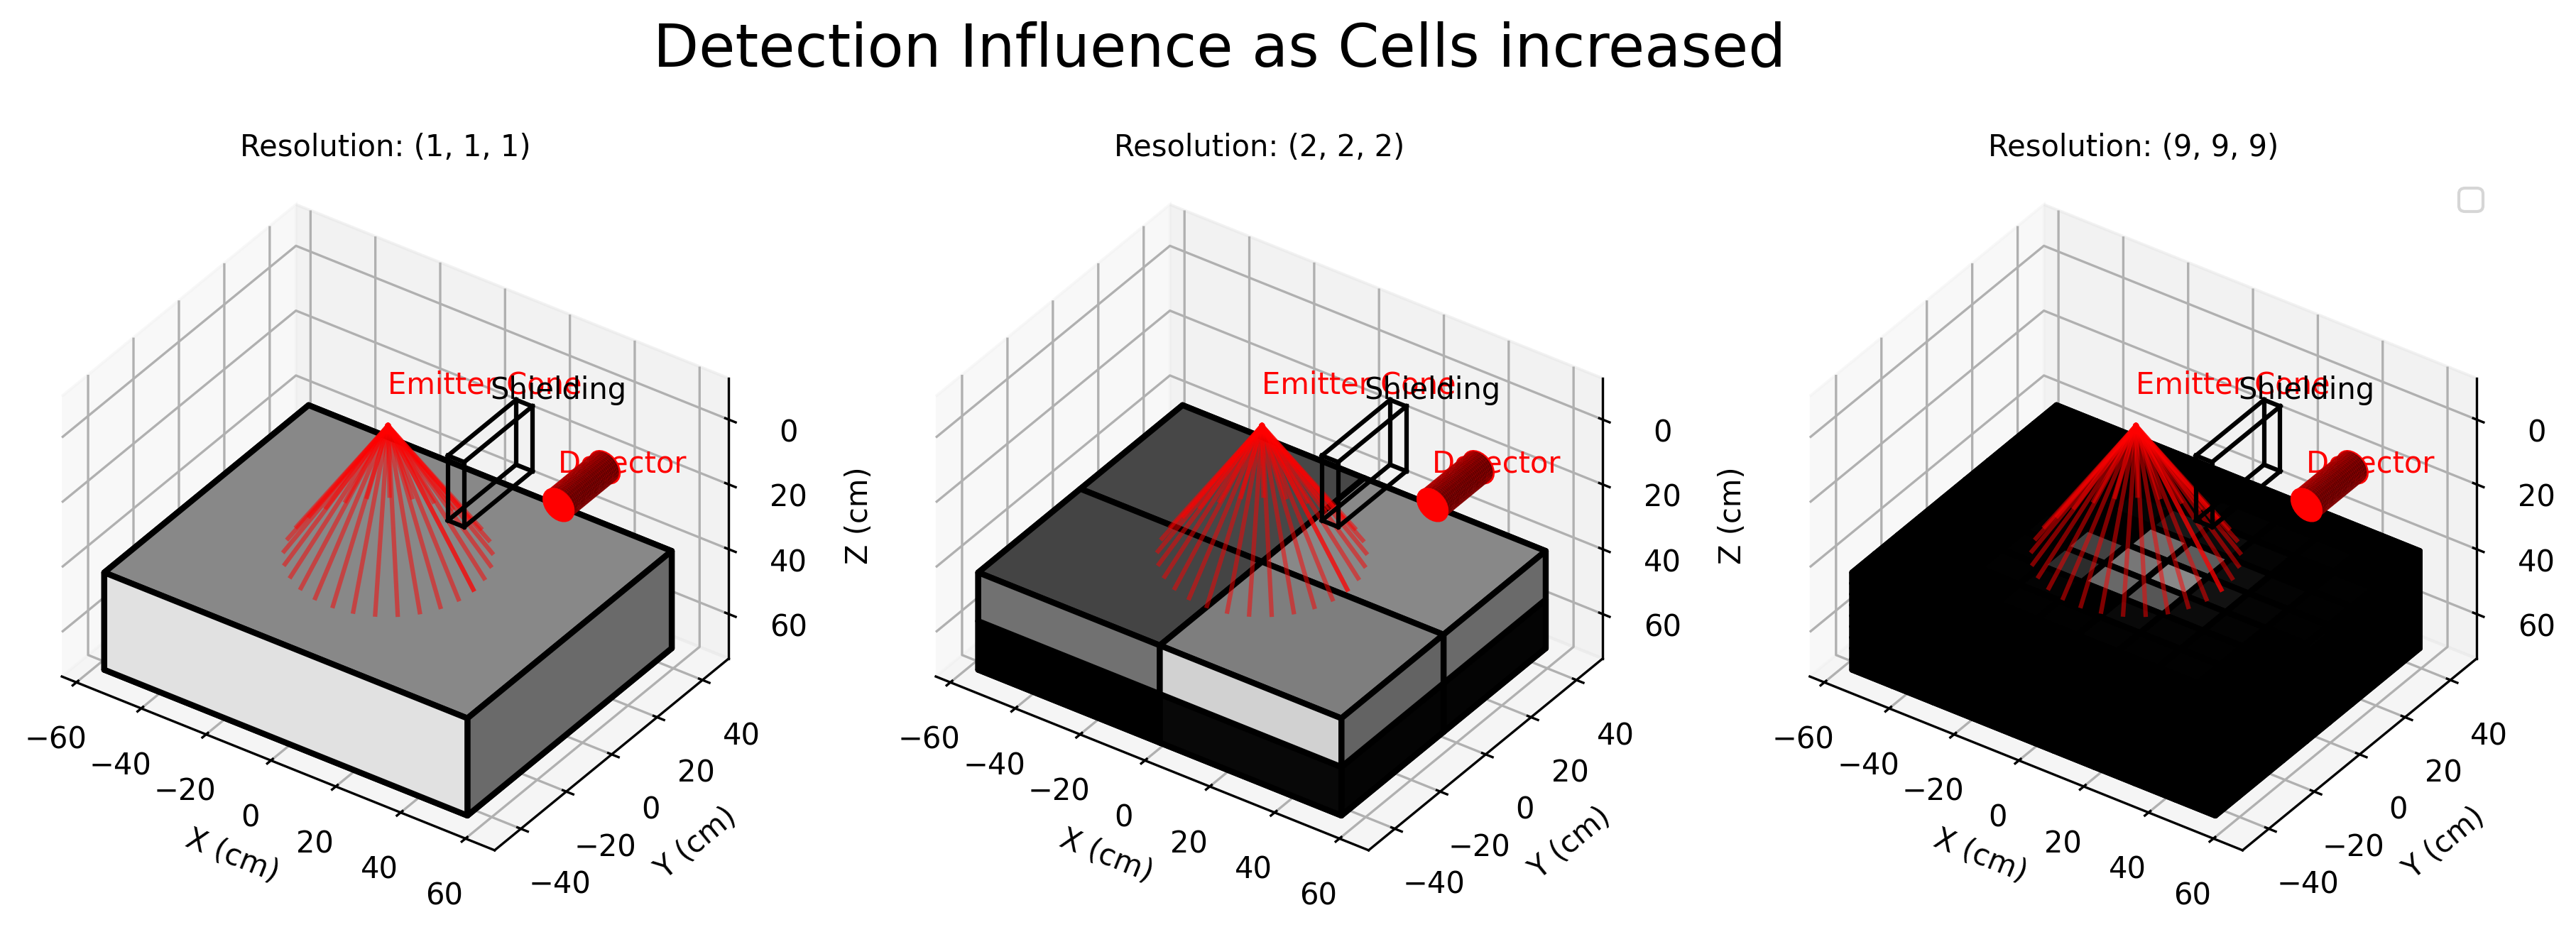
\includegraphics[width=1\linewidth]{../Figures/MCNP/CellRatioMesh.png}
\end{center}
\end{figure}
\begin{enumerate}
\item Treat mesh cells as independent
\item CU card: bins tally by cell of interaction
\item Allows investigation of where detections originate
\end{enumerate}
\end{frame}
\begin{frame}{Cell clouds}
\begin{figure}[Cell Clouds]
\begin{center}
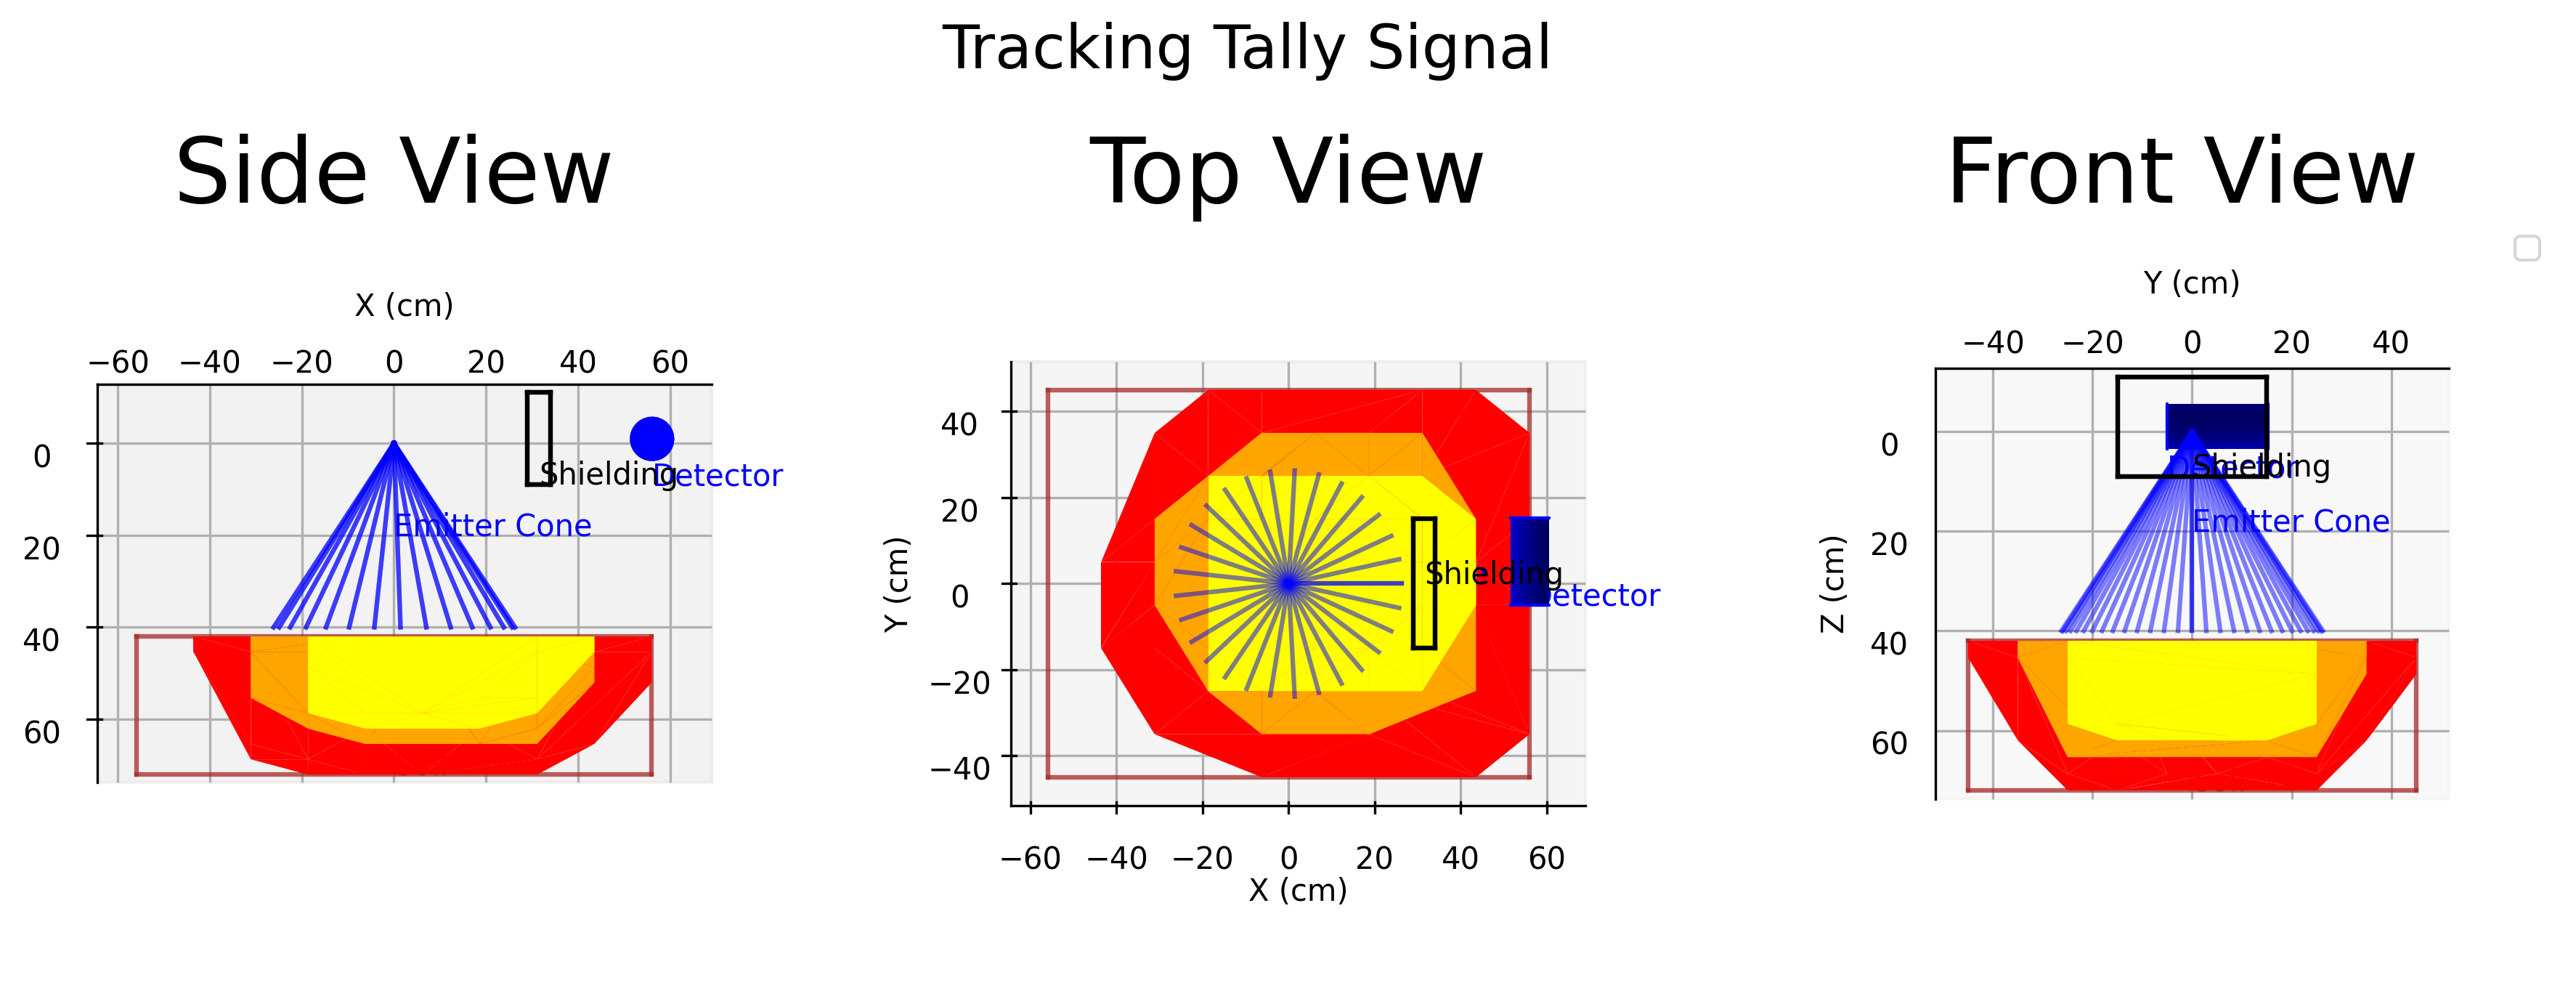
\includegraphics[width=1\linewidth]{../Figures/MCNP/CellClouds.png}
\end{center}
\end{figure}
\end{frame}
\begin{frame}{Range measurement}
\begin{figure}[Gradient Weighed Avg vs Homogeneous Avg]
\begin{center}
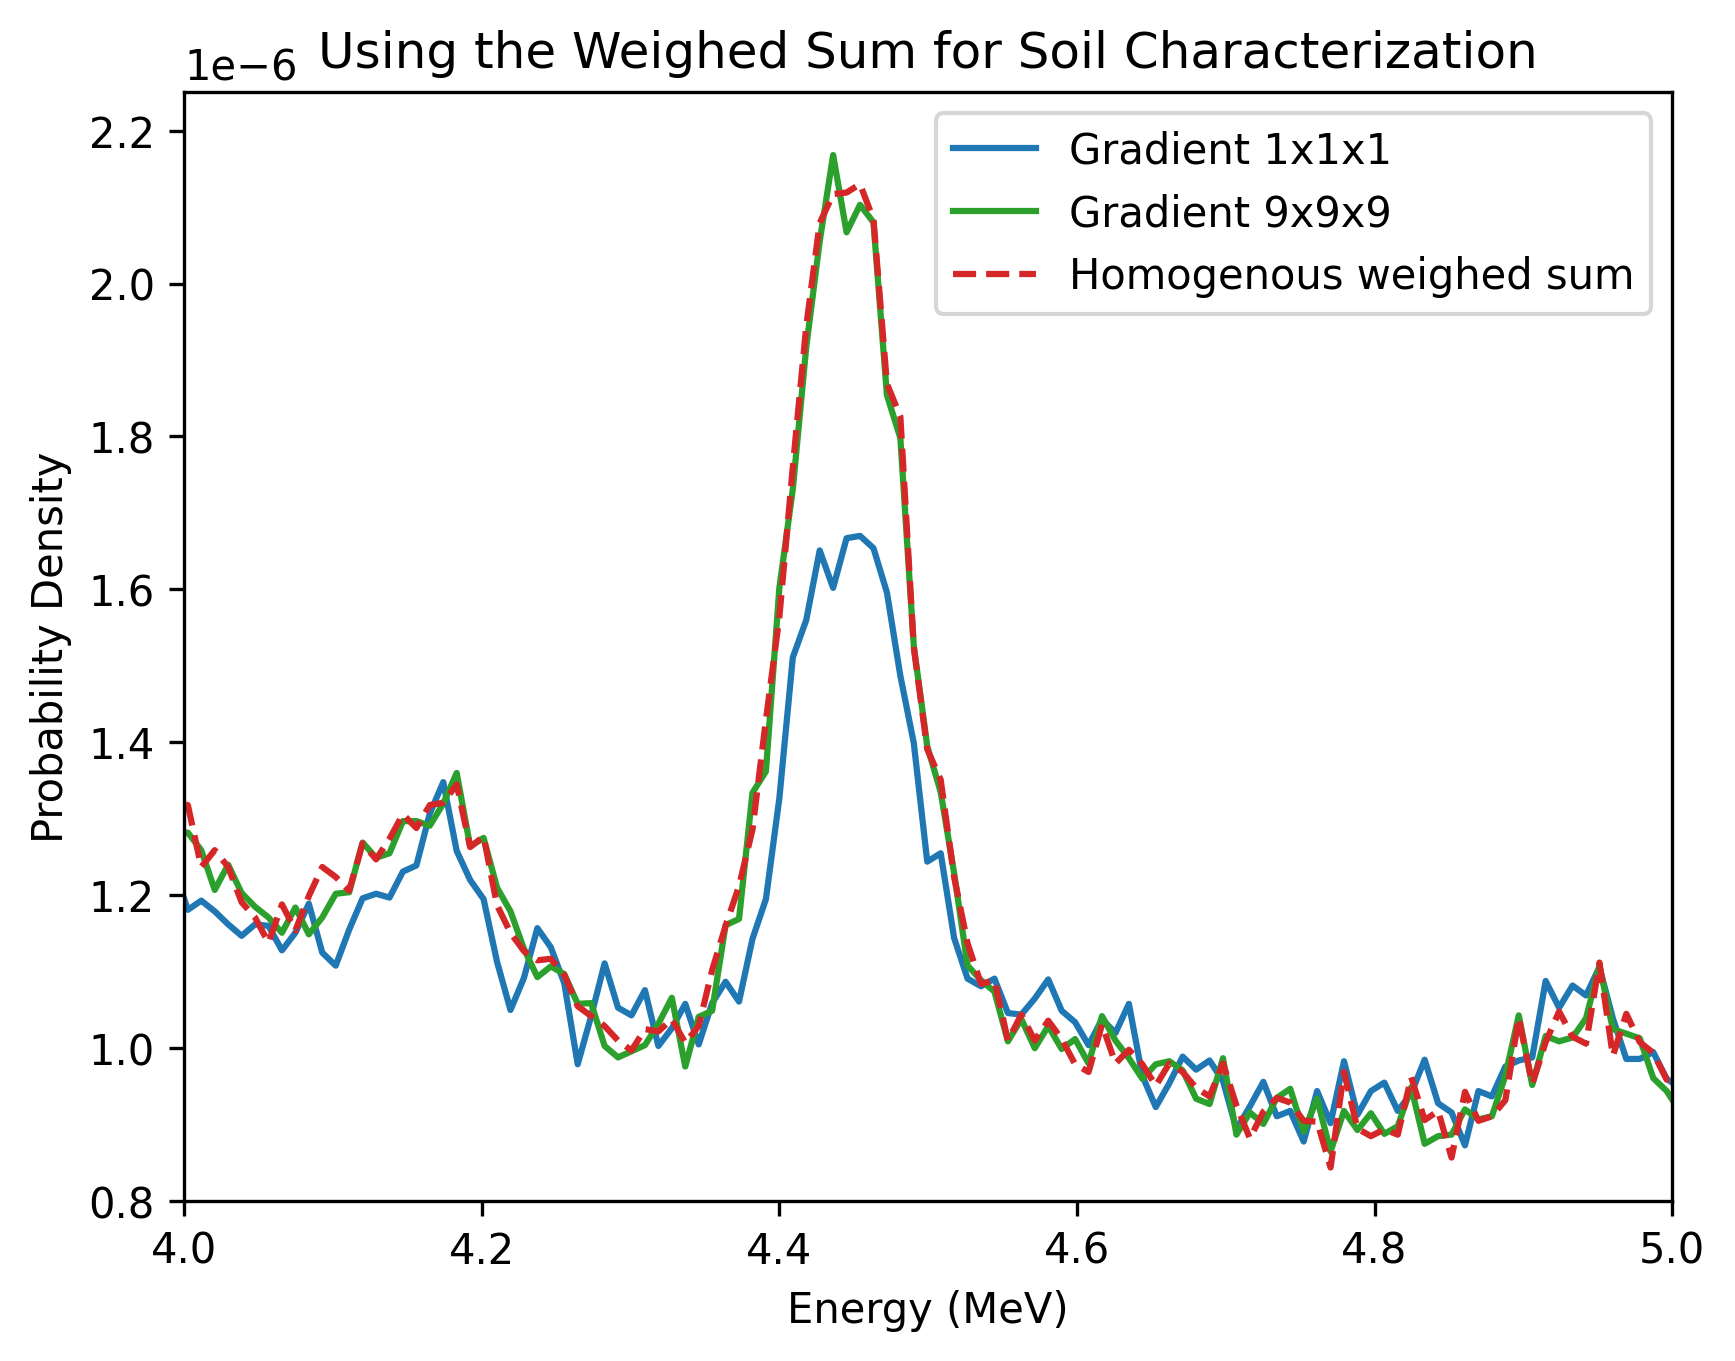
\includegraphics[width=1\linewidth]{../Figures/MCNP/GradientWeighedAvgvsHomogeneousAvg.png}
\end{center}
\end{figure}
\begin{enumerate}
\item Example: measure energy deposition in detector, binned by mesh cell
\item Weighted sum of tallies per bin
\end{enumerate}
\end{frame}
\begin{frame}{Usage Example}
\begin{figure}[Detector Direction to Measured Density]
\begin{center}
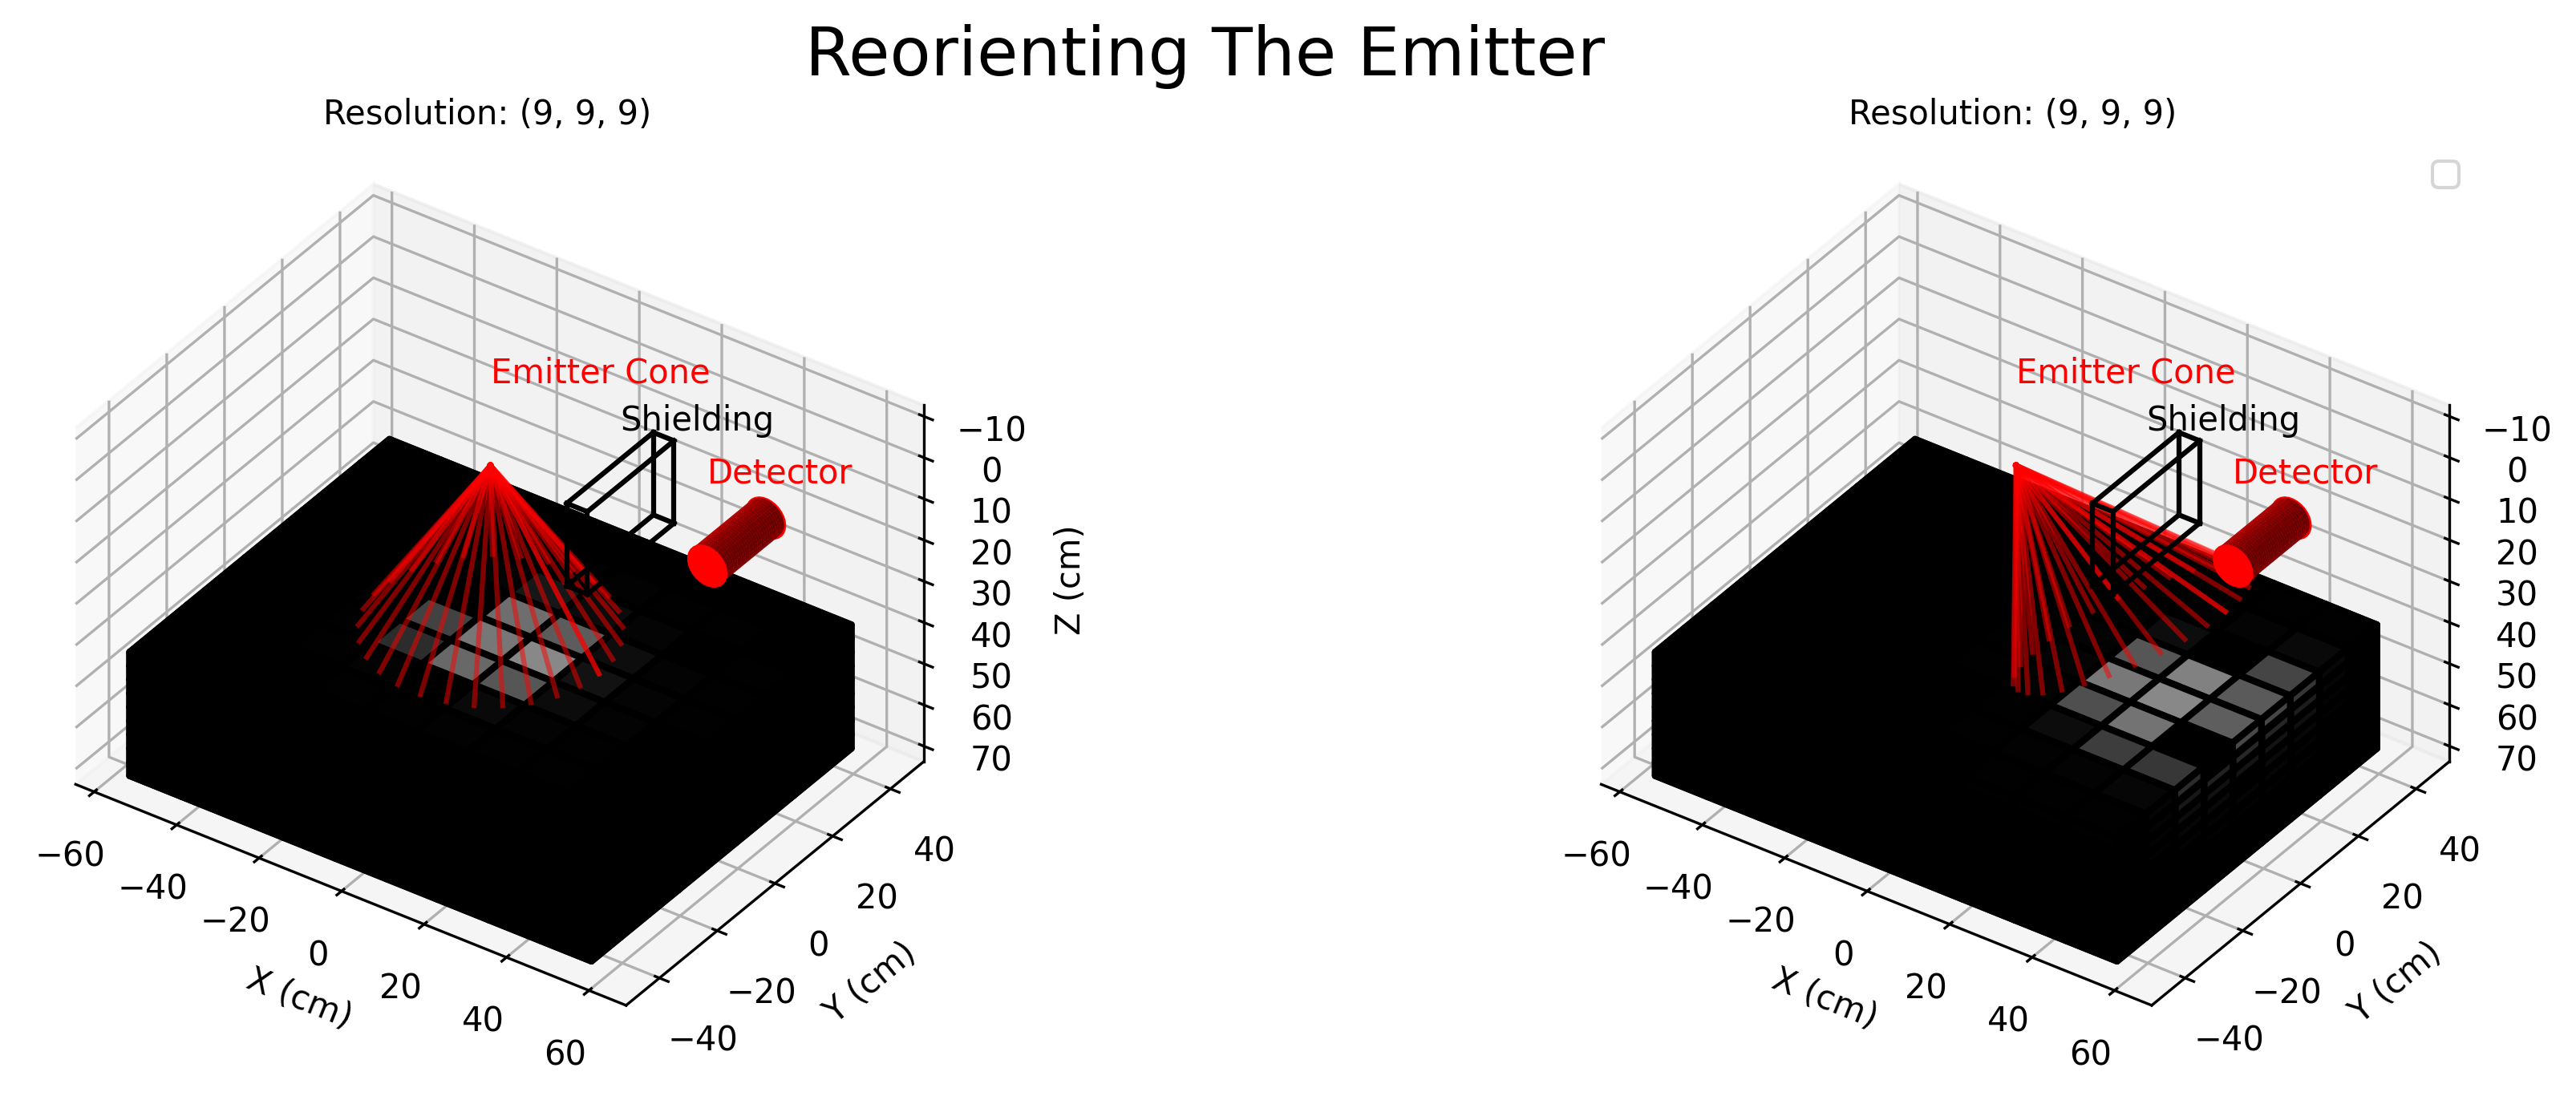
\includegraphics[width=1\linewidth]{../Figures/MCNP/DetectorDirectiontoMeasuredDensity.png}
\end{center}
\end{figure}
\begin{enumerate}
\item When machine design changes, simulate new detection results
\item Range can be re-evaluated
\item Example: pointing emitter under detector changes detection range
\end{enumerate}
\end{frame}
\section{Conclusion}
\begin{frame}{Summary}
\begin{enumerate}
\item Mesh cells allow for detailed soil modeling in MCNP
\item Enables accurate simulation of in situ spectroscopy
\item Helps understand detection range and sensitivity
\end{enumerate}
\end{frame}
\begin{frame}{Future Work}
\begin{enumerate}
\item Further refine mesh resolution for improved accuracy
\item Explore additional soil characteristics (hydration)
\item Accurate comparison with core harvesting results
\end{enumerate}
\end{frame}
\begin{frame}{Code}
\end{frame}
\begin{frame}{Acknoledgements}
\end{frame}
\begin{frame}{References}
\end{frame}
\begin{frame}{References}%[allowframebreaks] if too many references
    \renewcommand*{\bibfont}{\footnotesize}
    \bibliography{ref}
    \bibliographystyle{apalike}
    % \tiny\bibliographystyle{alpha}
\end{frame}

\end{document}